\section{Implementation}
\label{netqasm:sec:implementation}

\todo{Re-create Figures 8, 9 and 10 from netqasm paper?}

\subsection{Interface between \ac{CNPU} and \ac{QNPU}}
Here we explain the flow of messages between the \ac{CNPU} and the \ac{QNPU}.
The \ac{CNPU} starts by declaring the registration of an application, including resource-requirements for the application.
After this, the \ac{CNPU} sends some number of subroutines for the \ac{QNPU} to execute before declaring the application is finished.
See \cref{fig:message_sequence} for a sequence diagram and below for a definition of the messages.
In \cref{netqasm:sec:language} we will describe in more details the content of the subroutines and the format of instructions.
The \ac{QNPU} returns to the \ac{CNPU} an assigned application ID for the registered application and returns data based on the subroutines executed.

The \ac{CNPU} and the \ac{QNPU} are assumed to run independently and in parallel.
For example, while a subroutine is being executed by the \ac{QNPU}, the \ac{CNPU} could in principle do other operations, such as heavy processing or communication with another node.

\begin{figure}
      \centering
      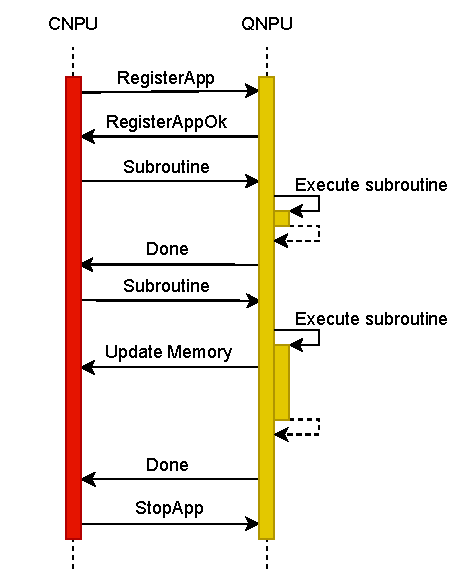
\includegraphics[width=0.6\linewidth]{figures/netqasm/message-flow.pdf}
      \caption{Flow of messages between the \ac{CNPU} and the \ac{QNPU}.}
      \label{fig:message_sequence}
\end{figure}

\Cref{fig:message_sequence} shows an example of a message exchange between the \ac{CNPU} and the \ac{QNPU}.
The content of these messages is further detailed in~\cref{netqasm:sec:app-messages}.



\subsection{The language}
\label{netqasm:sec:language}
The syntax and structure of \ac{NetQASM} resemble that of classical assembly languages, which in turn inspired the various QASM-variants for quantum computing~\cite{cross2017openqasm, khammassi2018cqasm, fu2019eqasm, liu2017fqasm}.

A \ac{NetQASM}-instruction is formed by an instruction name followed by some number of operands:
\begin{nqcode}
      instr operands
\end{nqcode}
where \nq{instr} specifies the instruction, for example \nq{add} to add numbers or \nq{h} to perform a Hadamard.
The \nq{operands} part consists of zero or more values that specify additional information about the instruction, such as which qubit to act on in the case of a gate instruction.
Instructions and operands are further specified in~\cref{netqasm:sec:operands}.

\subsection{Instructions}
\label{netqasm:sec:instructions}
There are eight groups of instructions in the \textbf{core} of \ac{NetQASM}.
Also summarized in \cref{fig:instructions}, these are:
\begin{itemize}
      \item \textbf{Classical:} Classical arithmetic on integers.
      \item \textbf{Branch:} Branching operations for performing conditional logic.
      \item \textbf{Memory:} Read and write operations to classical memory (register and arrays).
      \item \textbf{Allocate:} Allocation of qubits and arrays.
      \item \textbf{Wait:} Waiting for certain events. This can for example be the event that entanglement has been generated by the network stack.
      \item \textbf{Return:} Returning classical values from the \ac{QNPU} to the \ac{CNPU}.
            In our implementation we implement this by having the \ac{QNPU} write to the shared memory so that the \ac{CNPU} can access it.
      \item \textbf{Measurement:} Measuring a qubit.
      \item \textbf{Entanglement:} Creating entanglement with a remote node using the quantum network stack.
\end{itemize}

% \begin{figure}
%       \centering
%       \begin{tikzpicture}[node distance=12pt,
%                   flavour-box/.style={rectangle, rounded corners, fill=#1!30, align=center, yshift=-1.8cm,
%                               draw=black,
%                               minimum height=3cm, minimum width=(\x2-\x1-\pgflinewidth-12pt)/4},
%                   flavour-box/.default=green,
%                   group-box/.style={rectangle, rounded corners, minimum width=3cm, minimum height=1cm, text centered, draw=black, align=center},
%             ]
%             % Instruction groups
%             \node (classical) [group-box, fill=Cyan] {\textbf{Classical:}\\add, sub\\addm, subm};
%             \node (branch) [group-box, right=of classical, fill=LimeGreen] {\textbf{Branch:}\\jmp, bez, bnz,\\beq, bne, blt, bge};
%             \node (memory) [group-box, right=of branch, fill=BlueGreen] {\textbf{Memory:}\\set, store, load,\\undef, lea};
%             \node (allocate) [group-box, right=of memory, fill=Melon] {\textbf{Allocate:}\\array, qalloc, qfree};
%             \node (wait) [group-box, below=of classical, fill=SpringGreen] {\textbf{Wait:}\\wait\_all, wait\_any,\\wait\_single};
%             \node (return) [group-box, right=of wait, fill=Orange] {\textbf{Return:}\\ret\_reg, ret\_arr};
%             \node (measurement) [group-box, right=of return, fill=Lavender] {\textbf{Measurement:}\\meas};
%             \node (entanglement) [group-box, right=of measurement, fill=Orchid] {\textbf{Entanglement:}\\create\_epr, recv\_epr};

%             % Core
%             \node (core) [rectangle, above=of $(branch)!0.5!(memory)$, yshift=20pt] {\textbf{Core}};
%             \begin{scope}[on background layer]
%                   \node (core-bg) [fill=black!10, draw=black, rounded corners, inner sep=12pt,
%                         fit={(core) (classical) (branch) (memory)
%                                     (allocate) (wait) (return) (measurement) (entanglement)}] {};
%             \end{scope}

%             % Flavours
%             \node (flavours) [below=of core-bg, yshift=5pt] {\textbf{NetQASM flavors:}};
%             \path let
%             \p1 = (wait.west), \p2=(entanglement.east)
%             in node (vanilla) [flavour-box, below=of $(\p1)!1/8!(\p2)$]
%                   {\textbf{Vanilla flavor:}\\init,\\x, y, z,\\h, s, k, t,\\rot\_x, rot\_y, rot\_z,\\cnot, cphase};
%             \path let
%             \p1 = (wait.west), \p2=(entanglement.east)
%             in node (nv) [flavour-box, below=of $(\p1)!3/8!(\p2)$]
%                   {\textbf{NV flavor:}\\init,\\rot\_x, rot\_y, rot\_z,\\cx\_dir, cy\_dir};
%             \path let
%             \p1 = (wait.west), \p2=(entanglement.east)
%             in node (ti) [flavour-box, below=of $(\p1)!5/8!(\p2)$]
%                   {\textbf{TI flavor:}\\\dots};
%             \path let
%             \p1 = (wait.west), \p2=(entanglement.east)
%             in node (other-flavour) [flavour-box, below=of $(\p1)!7/8!(\p2)$, path fading=east]
%                   {\textbf{\dots}};
%       \end{tikzpicture}
%       \caption{The \textbf{core} of \ac{NetQASM} consists of eight groups of
%             instructions. The quantum gates are defined as a set of software-visible
%             gates part of a \ac{NetQASM} \textbf{flavor}. The \textbf{vanilla flavor}
%             is the unique platform-independent \ac{NetQASM} \textbf{flavor} of
%             \ac{NetQASM}, which can be used by a compiler.}\label{fig:instructions}
% \end{figure}

Quantum gates are specific to a \ac{NetQASM} \textbf{flavor} and given as a set of software-visible gates of a given platform, see \cref{netqasm:sec:design_considerations}.
There is a single platform-independent \ac{NetQASM} \textbf{flavor} which we call the \textbf{vanilla flavor}, see \cref{fig:instructions}.
The \textbf{vanilla flavor} can be used as an intermediate representation for a compiler.


\subsection{Compilation}
Although application programmers could write \ac{NetQASM} subroutines manually, and let their (classical) application code send these subroutines to the \ac{QNPU}, it is useful and more user-friendly to be able to write quantum internet applications in a higher level language, and have the quantum parts compiled to \ac{NetQASM} subroutines automatically.
For this, we use the compilation steps depicted in \cref{fig:comp_chain}.
The format and compilation of the higher-level programming language is not part of the \ac{NetQASM} specification.
However, we do provide an implementation in the form of an SDK, see \cref{netqasm:sec:python-sdk}.

% \tikzstyle{box} = [rectangle, rounded corners, minimum width=6cm, minimum height=1cm, text centered, draw=black]
% \tikzstyle{select} = [rectangle, dotted, draw=blue, very thick, inner sep=0.2cm]
% \tikzstyle{arrow} = [thick,->,>=stealth]
% \begin{figure*}
%       \centering
%       \begin{tikzpicture}[node distance=2cm]
%             \node (higher) [box, fill=red] {Higher-level programming language};
%             \node (hybrid) [box, below of=higher, fill=red] {Hybrid quantum-classical program};
%             \node (netqasm-unop) [box, below of=hybrid, fill=black!10!orange] {NetQASM (vanilla flavor)};
%             \node (netqasm-op1) [box, below of=netqasm-unop, fill=black!10!yellow] {NetQASM (HW flavor)};
%             \node (netqasm-op2) [box, below of=netqasm-op1, fill=black!10!yellow, yshift=-1cm] {NetQASM (HW flavor)};
%             % \node (semi-phys) [box, below of=netqasm-op2, fill=black!30!green] {Semi-physical instructions};
%             % \node (phys1) [box, below of=netqasm-op2, fill=black!30!green] {Physical instructions};
%             % \node (phys2) [box, below of=phys1, fill=black!30!green] {Physical instructions};
%             % text descriptions
%             \node[anchor=west,inner sep=3pt,text width=6cm] at ($(higher.east) + (15pt,0)$) {Full application, written by a programmer (e.g. Python)};
%             \node[anchor=west,inner sep=3pt,text width=6cm] at ($(hybrid.east) + (15pt,0)$) {Full application, multiple subroutines compiled together, including also classical logic at application level};
%             \node[anchor=west,inner sep=3pt,text width=6cm] at ($(netqasm-unop.east) + (15pt,0)$) {Virtual qubits part of allocated unit-module, abstract gates, single subroutine};
%             \node[anchor=west,inner sep=3pt,text width=6cm] at ($(netqasm-op1.east) + (15pt,0)$) {Same as above except for software-visible gates (platform-dependent)};
%             \node[anchor=west,inner sep=3pt,text width=6cm] at ($(netqasm-op2.east) + (15pt,0)$) {Input from above};
%             % \node[anchor=west,inner sep=3pt,text width=6cm] at ($(phys1.east) + (15pt,0)$) {Physical qubits, native gates};
%             % \node[anchor=west,inner sep=3pt,text width=6cm] at ($(phys2.east) + (15pt,0)$) {Input from above};
%             % arrows
%             \draw [arrow] (higher) -- node[anchor=east] {} (hybrid);
%             \draw [arrow] (hybrid) -- node[anchor=east] {(multiple subroutines)} (netqasm-unop);
%             \draw [arrow] (netqasm-unop) -- node[anchor=east] {(heavy compiling)} (netqasm-op1);
%             \draw [arrow] (netqasm-op1) -- node[anchor=east] {} (netqasm-op2);
%             % \draw [arrow] (netqasm-op2) -- node[anchor=east] {} (phys1);
%             % \draw [arrow] (phys1) -- node[anchor=east] {} (phys2);
%             % boxes
%             \node (compilation) [select,fit={($(hybrid.west) + (-5pt,0)$) ($(hybrid.north) + (0,8pt)$) (netqasm-unop) (netqasm-op1)}] {};
%             \node[anchor=north west,inner sep=3pt] at (compilation.north west) {Compilation};
%             \node (applayer) [select,fit={($(higher.north) + (0,8pt)$) (compilation)}] {};
%             \node[anchor=north west,inner sep=3pt] at (applayer.north west) {Application layer};
%             \node (qnpu) [select,fit={($(netqasm-op2.north) + (0,8pt)$) (netqasm-op2)}] {};
%             \node[anchor=north west,inner sep=3pt] at (qnpu.north west) {QNPU};
%             % \node (qdevice) [select,fit={($(phys2.north) + (0,8pt)$) (phys2)}] {};
%             % \node[anchor=north west,inner sep=3pt] at (qdevice.north west) {QDevice};
%       \end{tikzpicture}
%       \caption{Compilation steps from higher-level programming language, to the
%             \ac{NetQASM} \textbf{flavor} exposed by the specific platform. What is
%             contained at each level is further specified to the right of the
%             diagram.}
%       \label{fig:comp_chain}
% \end{figure*}
